\chapter{Systèmes hydrogénoïdes: structures fines et hyperfines}

\section{Effets relativistes et structure fine}
\subsection{L'équation de Dirac}
Soit l'équation de Schrödinger dépendante du temps
\begin{equation}
i \hbar \frac{\partial}{\partial t} \Psi = H \Psi 
\hspace*{3cm} \mbox{lin\'eaire en}~\partial/\partial t !
\end{equation}
\textsc{Dirac} aimait la dépendance temporelle linéaire de cette équation mais il n'aimait pas le 
$p^2/2m$ se cachant dans $T$, soit un terme non-linéaire. Il y avait donc un déséquilibre entre 
le temps et les trois composante d'espace ce qui ne plaisait pas (il y avait de plus pas mal 
d'arguments montrant que Schrödinger ne suffisait pas). Il était nécessaire de tout mettre sur
le même pied
\begin{equation}
(x,y,z,t) = (x_1,x_2,x_3, x_0 \equiv ct) ~\mbox{sur le m\^eme pied}
\end{equation}
Pour se faire, il faut que $H$ soit linéaire en les dérivées d'espace $\partial/\partial x_k$. 
Dirac a su montrer qu'en utilisant une fonction d'onde à quatre composantes, tout se déroulait 
correctement.
\begin{equation}
\Psi = \left(
\begin{array}{c} \Psi_1 \\ \Psi_2 \\ \vdots \\ 
\Psi_4 \end{array}
\right)
\end{equation}
Cette fonction d'onde doit être fonction propre d'un Hamiltonien linéaire en les variable $p$. Il a 
proposé
\begin{equation}
H = c \; \mbox{\boldmath $ \alpha $} \cdot {\bf p}
  + \beta \; mc^2
\end{equation}
Qui est bien linéaire en les variables d'espaces car $p$ apparaît à la place de $p^2$. Pour des raisons
dimensionnelle, il est nécessaire d'effectuer la multiplication par $\alpha$. Notons que, pour garder
la linéarité, $(\alpha^1, \alpha^2, \alpha^3, \beta)$ sont indépendant de $({\bf r},t,{\bf p})$. Grâce
à la présence du $\beta$, on peut également décrire l'antimatière. Écrivons $H\psi = E\psi$
\begin{equation}
(E - c \; \mbox{\boldmath $ \alpha $} \cdot {\bf p}
  - \beta \; mc^2 ) \Psi = 0
\end{equation}
Développons
\begin{equation}
i \hbar \frac{\partial}{\partial t} \Psi =
- i \hbar  c \mbox{\boldmath $ \alpha $} \cdot \mbox{\boldmath $ \nabla $} \Psi +  \beta \; mc^2  \Psi
\end{equation}
Injectons les quatre composante de la fonction d'onde
\begin{equation}
i \hbar \frac{\partial}{\partial t} \Psi_i = -i \hbar c 
\sum_{j=1}^4 \sum_{k=1}^3 \alpha_{ij}^k 
\frac{\partial}{\partial x_k} \Psi_j 
+ \sum_{j=1}^4 \beta_{ij} mc^2 \Psi_j,\qquad (i=1,2,3,4)
\end{equation}
Ceci exprime la variation d'une des quatre composante comme un couplage avec toutes les autres 
composantes. Les termes diagonaux vont se coupler (somme sur $j$) mais il y a une seconde somme
(sur $k$) portant sur les trois composantes de l'impulsion. Le $\alpha^k_{ij}$ est est ainsi une 
matrice. Bien sûr, s'inspirant de Klein-Gordon, Dirac a imposé l'hermiticité de $H$ et fait en sorte
que l'on puisse retomber sur son équation.\\

Au risque de se répéter, nous sommes dans un espace 4D où $\alpha$ est une matrice à quatre 
composantes "cachée" par $\vec \sigma$, les matrices de \textsc{Pauli}. On est alors forcée de 
constater que le spin est "inclus" dans l'équation de \textsc{Dirac}
\begin{equation}
\mbox{\boldmath $ \alpha $} = 
\left( \begin{array}{cc} 0 & \mbox{\boldmath $ \sigma $} \\
\mbox{\boldmath $ \sigma $} & 0 \end{array} \right),\qquad\qquad\qquad
\beta = 
\left( 
\begin{array}{cc} I & 0 \\
0 & - I    \end{array} \right)
\end{equation}

Jusqu'ici, nous ne savons pas comment se comporte une particule chargée munie d'un spin dans un 
champ électromagnétique. Pour en décrire le comportement, il suffit d'effectuer la substitution
$\vec p \to \vec{p}-q\vec{A}$ où $\vec A$ est le potentiel vecteur. On obtient alors
\begin{equation}
H = 
c  \mbox{\boldmath $ \alpha $} \cdot  ( {\bf p} - q {\bf A} )
+ q \Phi + \beta m c^2
\end{equation}
En étudiant les solutions stationnaire de la forme $\Psi ({\bf r},t) = \chi({\bf r}) e^{-iEt/ \hbar}$,
on en tire l'énergie
\begin{equation}
E \chi({\bf r}) =
[ - i \hbar  c \mbox{\boldmath $ \alpha $} \cdot \mbox{\boldmath $ \nabla $}
- c q \mbox{\boldmath $ \alpha $} \cdot {\bf A} + q \Phi + \beta mc^2 ] \chi({\bf r})
\end{equation}
où $\DS \chi ({\bf r}) \equiv \left( \begin{array}{c}
 \psi({\bf r}) \\ \eta({\bf r}) \end{array} \right)$.\\


Considérons un \textbf{champ central} ($\vec{A}=\vec0$). Le potentiel vaut alors $V(r)=q\Phi(r)$ de
sorte que l'on puisse écrire
\begin{equation}
H = 
c  \mbox{\boldmath $ \alpha $} \cdot  {\bf p}
 + \beta m c^2 + V(r)
\end{equation}
L'Hamiltonien non relativiste commutait (impliquant une invariance) avec $\vec{L^2}$ et $L_z$ et de
même pour le spin. La mauvaise nouvelle c'est que ceci n'est plus vérifié ici
\begin{equation}
[H,\vec{L}^2] \neq 0,\qquad\qquad\qquad [H,\vec{S}^2] \neq 0
\end{equation}
Cette non-commutation vient du fait que le $H_{rel}$ dépend du spin via $\alpha$ (qui contient 
$\vec \sigma$, les matrices de \textsc{Pauli}) tandis que la non commutation avec le moment cinétique
orbital vient du fait que $H$ contient $\vec{L}$ et non plu $\vec{L}^2$.\\

Cependant, bonne nouvelle, l'Hamiltonien commute avec le \textbf{moment angulaire total}
\begin{equation}
{\bf J} = {\bf L} + {\bf S} \Rightarrow [ {\bf J}, H ] = 0
\Rightarrow [H, {\bf J}^2] = 0
\end{equation}
Ceci permet de retrouver la relation de commutation $[ H , J_z ] = 0 \Rightarrow ~\mbox{EOC}~ = \{
{\bf J}^2, J_z \}$. Les vecteur/valeurs propres sont donnés par 
\begin{equation}
 \left\{ \begin{array}{l}
{\bf J}^2 \chi_{j,m_j} ({\bf r}) = j(j+1) \hbar^2 \chi_{j,m_j} ({\bf r}) \\
J_z \chi_{j,m_j} ({\bf r}) = m_j \hbar \chi_{j,m_j} ({\bf r}) 
\end{array} \right.
\end{equation}
Les problèmes de Schrödinger viennent d'un couplage mais on se rend ici compte que c'est plus 
fondamental que ça. De même, avec $\vec{J}^2$ on sent venir le couplage \textit{spin-orbite} avec
un facteur $2\vec{L}.\vec{S}$ qui va apparaître.\\

Résumons
\begin{equation}
H = 
c  \mbox{\boldmath $ \alpha $} \cdot  {\bf p}
 + \beta m c^2 + V(r),\qquad\qquad
 \chi ({\bf r}) = \left( \begin{array}{c}
  \psi({\bf r}) \\ \eta({\bf r}) \end{array} \right)
\end{equation}
Avec les relations de commutations
\begin{equation}
[H, {\bf L}^2 ] \neq 0; \hspace*{1cm}  [H, {\bf S}^2 ] \neq 0;,\qquad\qquad\qquad
[H, {\bf J}^2 ] = [H, J_z] = 0
\end{equation}
Décrire un électron avec l'équation de \textsc{Dirac} est compliqué : on va y arriver à l'aide d'une
fonction à quatre composante. Nous allons l'écrire comme quelque chose qui \textit{ressemble} à un
spinneur de rang 2 mais qui n'en est pas un car chacune de ses deux composantes contiennent un peu
de spin \textit{up} et \textit{down}. Il y a donc bien en réalité quatre composantes
\begin{equation}
\chi_{E \kappa m_j} ({\bf r}) =\frac{1}{r} \left( \begin{array}{c}
 {\color{blue} P}_{E \kappa m_j}(r) \xi_{\kappa,m_j}(\theta, \phi) \\ 
 i {\color{red} Q}_{E \kappa m_j} (r)  \xi_{- \kappa, m_j (\theta, \phi)} 
\end{array} \right) 
\end{equation}
Inspectons les valeurs/vecteurs propres
\begin{equation}
\left\{
\begin{array}{l}
{\bf J}^2 \; \chi_{E \kappa m_j} ({\bf r}) = j(j+1) \hbar^2  \; \chi_{E \kappa m_j} ({\bf r})\\
J_z \; \chi_{E \kappa m_j} ({\bf r}) = m_j  \hbar \; \chi_{E \kappa m_j} ({\bf r}) \\
K \; \chi_{E \kappa m_j} ({\bf r}) = \kappa \; \chi_{E \kappa m_j} ({\bf r})
\end{array} \right.
\end{equation}
Où nous avons créer un opérateur $K$ de valeur propre $\kappa = \kappa = -(j+1/2)a$ où $a=\pm1$. 
Afin de comprendre l'intérêt de cet opérateur, considérons le tableau suivant
\begin{equation}
\begin{array}{lcccccc}
  & s_{1/2} & p_{1/2} & p_{3/2} & d_{3/2} & d_{5/2} & f_{5/2}  \\
j & 1/2 & 1/2 & 3/2 & 3/2 & 5/2 & 5/2 \\
l & 0 & 1 & 1 & 2 & 2 & 3 \\
a & +1 & -1 & +1 & -1 & +1 & -1 \\
\kappa & -1 & +1 & -2 & +2 & -3 & +3
\end{array}
\end{equation}
L'intérêt de la valeur propre $\kappa$ est qu'elle permet de désigner de façon unique un électron (
$j$ ou $l$ seul ne suffit pas à complètement caractériser un électron). Elle permettra également de
comprendre l'expression du vecteur propre décrit ci-dessus où l'on voit apparaître $\kappa$ dans la
première composante et $-\kappa$ dans la seconde.

\subsection{Couplage entre petite et grande composantes}
Ré-écrivons notre spinneur de rang 4
\begin{equation}
\chi_{E \kappa m_j} ({\bf r}) =\frac{1}{r} \left( \begin{array}{c}
 P_{E \kappa m_j}(r) \xi_{\kappa,m_j}(\theta, \phi) \\ 
 iQ_{E \kappa m_j} (r)  \xi_{- \kappa, m_j (\theta, \phi)} 
\end{array} \right)
\end{equation}
Ce qu'il faut comprendre, c'est que chacun des six $\kappa$ qui apparaissent est un mélange des 
harmonique. Afin de comprendre pourquoi il existe un tel couplage (on parlera de couplage entre 
la \textit{petite (Q) et la grande (P) composante}) existe, il faut regarder ce qui se cache dans
l'Hamiltonien. Par l'intermédiaire de $\alpha$, nous avons le produit suivant
\begin{equation}
\mbox{\boldmath $ \sigma $} \cdot {\bf p}
\left\{ \frac{F(r)}{r} \xi_{\kappa, m_j} (\theta, \phi) \right\}
= i \hbar \frac{1}{r} \left\{ \frac{dF}{dr} + \frac{\kappa F}{r} \right\}  \xi_{-\kappa, m_j} (\theta, \phi)\}
\end{equation}
Ceci nous renseigne sur l'application de $\vec{\sigma}.\vec{p}$ à une fonction radiale. On peut 
ré-écrire l'application de $H$ sur notre fonction propre
\begin{equation}
\left(
\begin{array}{cc}
mc^2 -E + V  &  -c \hbar \left( \frac{d}{dr} - \frac{\kappa}{r} \right) \\
 c \hbar \left( \frac{d}{dr} + \frac{\kappa}{r} \right) & -mc^2 -E + V 
\end{array} 
\right)
\left(
\begin{array}{c}
P_{E \kappa} (r) \\ Q_{E \kappa} (r) \end{array}
 \right) = 0
\end{equation}
Nous allons nous rendre compte que, dans cet algèbre, $P$ est couplé à $Q$ en développant cette
expression
\begin{equation}
\begin{array}{ll}
\DS\left[  \frac{d}{dr} + \frac{\kappa}{r}   \right] 
{\color{blue} P}_{E \kappa} (r)
&\DS= \frac{E + mc^2 - V(r)}{\hbar c} 
\DS{\color{red} Q}_{E \kappa} (r)\vspace{2mm}\\
\DS\left[  \frac{d}{dr} - \frac{\kappa}{r}   \right] 
{\color{red} Q}_{E \kappa} (r)
&\DS= - \frac{E - mc^2 - V(r)}{\hbar c} 
{\color{blue} P}_{E \kappa} (r)
\end{array}
\end{equation}
Il s'(agit d'une équation différentielle d'ordre 1 en $P$ et $Q$ dont nous avons besoin pour
décrire l'orbitale relativiste. Il existe ainsi bien un couplage radial. Nous avons séparer radialement en supposant une forme (fonction radiale * qqch($\theta,\phi$)) mais ce "quelque chose"
est beaucoup plus compliqué\footnote{Il est nécessaire d'utiliser les coefficients de CG pour écrire
le couplage spin-orbite}.\\
 
Pour s'en rendre compte, considérons un électron $2p$. Si $j=3/2, m_j = -1/2,-3/2,\dots$. Choisissons
$m_j = -1/2$. Déballons nos deux fonctions radiales $P$ et $Q$ (grande et petite composante)
\begin{equation}
\chi_{2p_{{3/2}, -1/2}} ({\bf r}) =\frac{1}{r} \left( \begin{array}{c}
 {\color{blue} P}_{2p_{3/2} }(r) \left(   +\sqrt{\frac{1}{3} } \right) Y_{1,-1} (\theta, \phi)\;  \alpha \\ 
 {\color{blue} P}_{2p_{3/2} }(r) \left(   +\sqrt{\frac{2}{3} } \right) Y_{1,0} (\theta, \phi)\;  \beta \\ 
 i {\color{red} Q}_{2p_{3/2} } (r) \left(   -\sqrt{\frac{3}{5} } \right) Y_{2,-1} (\theta, \phi)\;  \alpha  \\
  i {\color{red} Q}_{2p_{3/2} } (r)  \left(  + \sqrt{\frac{2}{5} } \right) Y_{2,0} (\theta, \phi)\;  \beta \end{array} \right)
\end{equation}
Examinons la première ligne. On retrouve $Y_{1,-1}$ ce qui est cohérent avec un électron $p$ ($l=1$)
et la projection vaut $m_l=1$ car l'égalité $j=l+s$ doit être respectée. Il reste comprendre pourquoi
le spin est \textit{up} (via $\alpha$). Rappelons-nous de la règle de sélection induite par les
coefficients de CG : $m_j=m_l+m_s$. Nous volons construire un état où $m_j = -3/2$. Comme nous avons
un électron $p$, $m_l$ peut valoir -1,0 ou 1. Il faut donc que $m_s=m_j-m_l$. Or comme $m_l=-1$ et 
$m_j=-1/2$ la projection du spin vaut $m_s=1/2$, soit un spin \textit{up}. Le spin étant \textit{down}
pour la seconde ligne, on retrouve bien du $\beta$.\\

La surprise est à la troisième ligne où l'on retrouve l'harmonique sphérique $Y_2$. Ceci vient du fait
que $l$ n'est plus un bon nombre quantique (mais il ne faut pas jeter les harmoniques sphériques pour
autant). La présence de $Y_2$ vient du fait que, dans la définition de $\chi$, $\kappa$ est renvoyé
en $-\kappa$.  Comme l'opérateur change (le signe) de $\kappa$, il va créer un mélange entre 
l'orbitale $p$ et $d$ comme le montre le tableau ci-dessus. Ceci explique la présence des harmoniques
$Y_2$ dans la description d'un électron $p$. Les racines apparaissant ne sont rien d'autres que les
coefficients de CB explicités (à cause du couplage \textit{spin-orbite}).


\newpage
\subsection{Spectre de Dirac}
	\begin{wrapfigure}[14]{l}{6cm}
	\vspace{-5mm}
	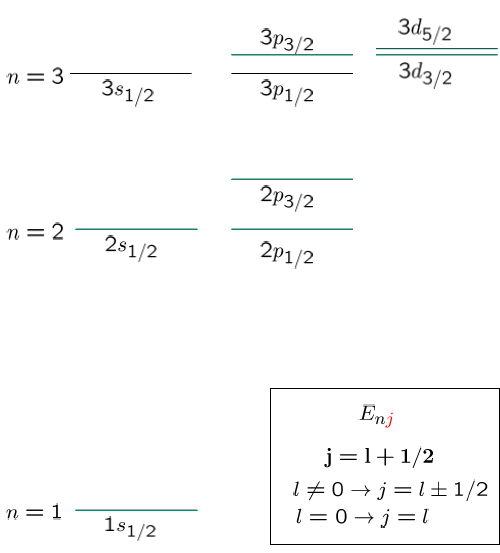
\includegraphics[scale=0.45]{ch2/image8}
	\captionof{figure}{ }
	\end{wrapfigure}
	
Sans surprise, l'énergie de \textsc{Dirac} dépend de $n$, mais aussi du nombre quantique $j$
\begin{equation}
E_{nj}^D = mc^2\times \left[ 1 + 
\left(
\frac{Z \alpha} {n-j-1/2 + [(j+1/2)^2 - Z^2 \alpha^2)^{1/2}}
\right) ^2  \right] ^{-1/2}
\end{equation}
Il s'agit de la solution analytique de \textsc{Dirac}. Afin de faire le lien avec 
\textsc{Schrödinger}, nous allons étudier le comportement de cette solution lorsque $Z\alpha$ n'est
pas trop important ou, autrement dit, lorsque les effets relativistes ne sont pas trop grands. 
Développons alors en puissance de $(Z\alpha)^2$
\begin{equation}
E_{nj}^D = mc^2= mc^2 \left[
1 - \frac{(Z \alpha)^2}{2 n^2} 
- \frac{(Z \alpha)^4}{2n^4} \left(
\frac{n}{j+1/2} - \frac{3}{4} \right) + \ldots \right]
\end{equation}\ \\
Bonne nouvelle : l'énergie relativiste de \textsc{Dirac} n'est autre que $mc^2$ et si on retire cette
énergie, il y a toujours une dépendance en $n$ et $j$. Il est donc possible d'exprimer, en faisant
cette soustraction, l'énergie non relativiste à laquelle s'ajoute des corrections proportionnelles
à l'énergie relativiste\footnote{Pour rappel, le solutions de l'équation de Schrödinger sont 
données par $E_n^{\mbox{NR}} =
- \frac{1}{2} \mu c^2 \frac{(Z \alpha)^2}{n^2} ; \hspace*{1cm}
{\color{red} \alpha = \frac{e^2}{(4 \pi \epsilon_0) 
\hbar c}}$.}
\begin{equation}
E_{n {\color{red} j}} = E^D_{nj} - mc^2 = E_n^{\mbox{NR}} \left[
1 + \frac{(Z \alpha)^2}{n^2} \left(
\frac{n}{{\color{red} j}+1/2} - \frac{3}{4} \right) + \ldots \right]
\end{equation}
Les corrections dépendent évidemment de $j$ et c'est rassurant car si $c\to \infty$, on retrouve
l'énergie non-relativiste qui n'est autre que la valeur propre de l'équation de \textsc{Schrödinger}.


\subsection{Fonctions radiales de Dirac}
Représentons l'orbitale $R$ de \textsc{Dirac}. Soit l'atome de $Hg^{79+}$ où 79 électrons ont été
arrachés de façon à former un système hydrogénoïde. En rouge, la \textit{grande composante} $P$ 
rappelle l'orbitale $2s$. On comprend également la désignation \textit{petite composante} à l'aide
de la courbe en vert représentant $Q$. Si $c\to\infty, Q\to 0$ et la petite composante s'éteint : on
retrouve l'expression de $P$ identique à celle trouvée avec \textsc{Schrödinger}. On peut remarquer
que ces deux composantes ne s'annulent pas au même rayon $r$. La somme des deux composantes ne 
s'annulera donc jamais : disparition de la structure noeudale.\\


On peut voir que l'effet non-relativiste n'est pas négligeable lorsque l'on représente la densité
$NR$ de \textsc{Schrödinger} $D_{n l}(r) = \vert P_{nl}(r) \vert^2 = r^2 R_{nl}(r) ^2$ et la 
densité $R$ de \textsc{Dirac} $D_{n \kappa}(r) = \vert P_{n \kappa}(r) \vert^2
+  \vert Q_{n \kappa}(r) \vert^2$.\\

Comme prévu, la densité ne s'annule jamais. On observe également une contraction de l'onde signifiant
une contraction de l'énergie de liaison. La structure ressemble cependant toujours à celle de 
\textsc{Schrödinger}. Cet effet est également présent dans d'autres orbitales (voir \textit{slide 
45}).


\begin{center}
	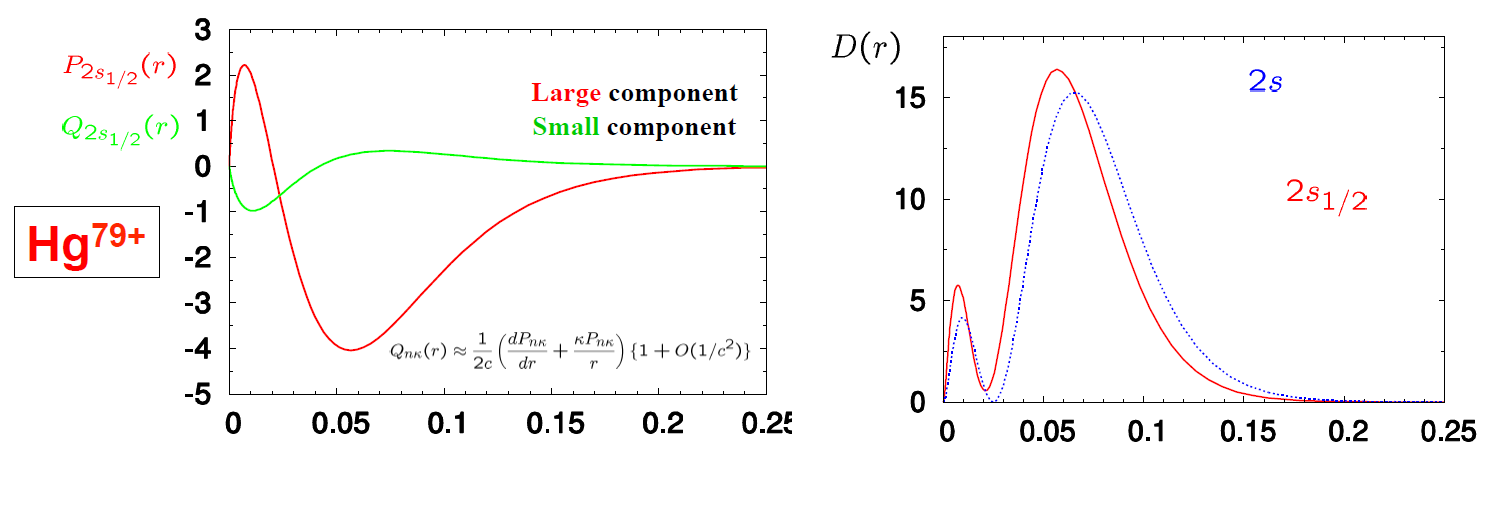
\includegraphics[scale=0.4]{ch1/image9}
	\captionof{figure}{ }
\end{center}


\subsection{Limite non relativiste de Dirac}
Il n'est pas possible d'ignorer les résultats obtenu par l'équation de \textsc{Dirac}. Cependant, 
il est possible d'essayer de "mimiquer" le spectre de \textsc{Dirac} en bye-passant la complexité
de son équation. L'idée est d'exprimer l'Hamiltonien de Dirac comme un de Schrödinger additionné à
une perturbation de sorte à pouvoir écrire $H \psi ({\bf r}) = E' \psi ({\bf r})$. \\

Les corrections proposées ci-dessous vont être correctes jusqu'à l'ordre $(v/c)^2$. Considérons un
potentiel central
\begin{equation}
\left\{
\begin{array}{l}
{\bf A } = 0 \\
q \Phi = - e \Phi = V(r) = -\frac{Ze^2}{(4 \pi \epsilon_0) r}
\end{array} \right.
\end{equation}
En mimiquant, on obtient
\begin{equation}
H = \frac{p^2}{2m} + V(r)- \frac{p^4}{8 m^3 {\color{red} c^2}} 
+ \frac{1}{2m^2 {\color{red} c^2}} \frac{1}{r}
  \frac{dV}{dr} {\bf L} \cdot {\bf S} 
 + \frac{\pi \hbar^2}{2 m^2 {\color{red} c^2 } }
  \left( \frac{Ze^2}{4 \pi \epsilon_0} \right) \delta( {\bf r} )
\end{equation}
où $V(r)$ est le potentiel d'interaction des protons, où l'on retruve une correction de \textit{masse
à l'énergie cinétique}
\begin{equation}
H^{\mbox{M}} = - \frac{p^4}{8 m^3 c^2}
\end{equation}
Une correction due à l'interaction \textit{spin-orbite}
\begin{equation}
H^{\mbox{s-o}} = + \frac{1}{2m^2 c^2} \frac{1}{r}
  \frac{dV}{dr} {\bf L} \cdot {\bf S} 
\end{equation}
Et une correction de \textit{Darwin}
\begin{equation}
H^{\mbox{D}} = 
 + \frac{\pi \hbar^2}{2 m^2 c^2 } 
  \left( \frac{Ze^2}{4 \pi \epsilon_0} \right) \delta( {\bf r} )
\end{equation}

La correction la plus parlante est l'interaction spin-orbite venant du fait que \textsc{Dirac} a 
forcé le couplage entre $\vec{L}$ et $\vec S$. Les deux autres corrections sont assez difficile à 
interpréter physiquement et il n'existe pas de consensus sur leur interprétation, nous n'y reviendrons
pas. Notons la signature relativiste de ces corrections via le facteur $1/c^2$. Le \textit{slide 47}
montre l'impact de ces différents corrections au sein de la couche $n=2$. Les \textit{slides 48} à
\textit{53} seront vus en séance d'exercices et ne sont pas repris ici (le but est de dériver
l'expression de l'énergie dû à la structure fine)\footnote{Lire notes personnelles \textit{slide 54}}.




\section{Lamb shift (1947)}
\subsection{Levée de la dégénérescence pour $j=1/2$}
La catastrophe (ou beauté) c'est que tout n'est pas prévu par l'équation de \textsc{Dirac}. En 
observant les niveaux $n=2$, \textsc{Lamb} a obtenu trois niveaux et non pas deux comme le 
prévoyait\textsc{Dirac} : il y a une levée de la dégénérescence pour $j=1/2$.\\

	\begin{wrapfigure}[9]{l}{6cm}
	\vspace{-5mm}
	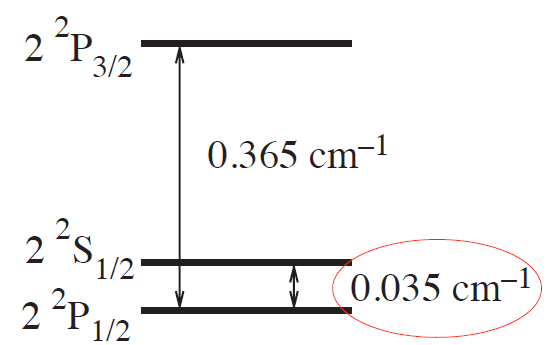
\includegraphics[scale=0.4]{ch1/image10}
	\captionof{figure}{ }
	\end{wrapfigure}
L'énergie dépend non seulement de $j$, mais peut-être bien de $n$ également. Il s'agit d'un effet 
plus fin que la structure fine, mais ce n'est pas la structure \textit{hyperfine} non plus. Il 
s'agit de la première manifestation pour un électron de l'électrodynamique quantique. Cet effet
est causé par les oscillations du vide\footnote{Si l'on admet que le vide sont des petits OH, on 
est forcée de constater que même à température nulle le système vibre encore ($E_v = \hbar\omega/2$.
Il existe donc un champ électromagnétique oscillant dans le fondamental que l'on nomme 
\textit{oscillation du vide du champ EM}.} que \textsc{Dirac} ne prend pas en compte. Or, un 
électron $2s$ ressent ces oscillation différemment qu'un électron $2p$ mais pour calculer ces 
déplacements, il faut se tapper un diagramme de \textsc{Feynman}.\\

L'énergie d'ionisation de l'hydrogène est d'à peu près 110 000 cm$^{-1}$. Ce déplacement de 
\textsc{Lamb} est d'à peu près 0.038 cm$^{-1}$ pour l'hydrogène mais peut atteindre 75 eV pour 
l'uranium.


\section{Structure hyperfine de l'hydrogène}
	\begin{wrapfigure}[14]{r}{7cm}
	\vspace{-5mm}
	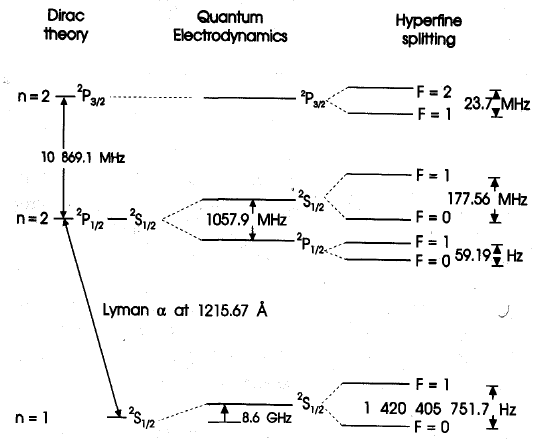
\includegraphics[scale=0.5]{ch1/image11}
	\captionof{figure}{ }
	\end{wrapfigure}
On s'intéresse ici à un effet nucléaire sur la structure électronique. Avec une résolution 
suffisamment fine, on s'aperçoit qu'il n'y a pas deux niveau pour $n=1$ mais quatre. Regardons
l'état fondamental $1s$ en Schrödinger qui devient $^2S_{1/2}$ dans Dirac\footnote{Le 2 en haut à 
gauche représente un \textit{doublet} car l'électron peut être dans deux états de spin (
$S=1/2, m_s =\pm1/2$ : \textit{up} et \textit{down}. Lorsque $S=1, m_s=-1,0,1$ et on parle de triplet.
De même lorsque $S=3/2$, $m_s = \pm 1/2, \pm 3/2$ et on parle de quadruplet, etc. }. \\

Cet effet s'observe même dans un cage de \textsc{Faraday} isolé de tout champ. Cependant, lorsque
l'on place un champ d'induction magnétique le niveau (pour $n=1$) $F=0$ donne un niveau tandis que
$F=1$ se divise en trois niveau (levée de dégénérescence). Il faut trouver quelque chose qui 
préserve l'invariance par rotation mais donnant un couplage\footnote{Si $F=2$, nous aurons 5 
valeurs.}. \\

Ce quelque chose c'est le noyau car le proton ($^1$H) possède un moment angulaire ; un spin noté
$I=1/2$. Il va y avoir un couplage entre $J$ (nature électronique) et $I$ (nature nucléaire)
\begin{equation}
{\bf F} = {\bf J} + {\bf I} \Rightarrow 
F = J+I, J+I-1, \ldots, \vert J-I \vert
\end{equation}
Notons que la théorie de l'électrodynamique quantique justifie un déplacement du fondamental mais
ne met pas en évidence un nouvelle structure. Cette dernière apparaît cependant bien lorsque
l'on \textit{regarde de plus près}. Remarque : $1GHz$ correspond à $\pm 10^{-6}$ eV ce qui n'est 
pas grand chose!\\

Pour chiffrer ces effets, on utilise le \textit{moment magnétique de spin $\mu_I$}, le 
\textit{magnéton de Bohr} $\mu_B$ et le \textit{magnéton nucléaire} $\mu_N$
\begin{equation}
\mbox{\boldmath $ \mu $}_I = g_I \mu_N {\bf I}/ \hbar,\qquad\qquad
\mu_B = \frac{e \hbar}{2m_e},\qquad\qquad
\mu_N = \frac{e \hbar}{2M_p} = \frac{m_e}{M_p} \mu_B
\end{equation}
Le moment nucléaire est colinéaire au moment magnétique : le rapport $\mu_N/\mu_B$ vaut à peu près
1836. La définition de $\vec F$ crée évidemment un nouvel \textsc{ecoc}.

\subsection{État fondamental $1s_{1/2}$}
Il existe des interactions avec le spin de l'électron. Dans l'état $1s$, nous avons 
${\bf J} = {\bf L} + {\bf S} = {\bf S}$. En définissant $\mbox{\boldmath $ \mu $}_S = -g_S \mu_B {\bf
S}/ \hbar$, on peut écrire un Hamiltonien décrivant cette interaction
\begin{equation}
H^{M1}_{\mbox{spin}} = - \mbox{\boldmath $ \mu $}_S \cdot 
{\bf B} = 2 \mu_B {\bf S} \cdot {\bf B} / \hbar
\end{equation}
Pour l'obtenir on travaillera avec le potentiel vecteur ${\bf A} ({\bf r}) = - \frac{\mu_0}{4 \pi}
\left[ \mbox{\boldmath $ \mu $}_I \times \mbox{\boldmath $ \nabla $} \left( \frac{1}{r} \right)
\right]$ avec lequel il est possible d'en tirer ${\bf B} = \mbox{\boldmath $ \nabla $} \times {\bf A}
= -\frac{\mu_0}{4 \pi} \left[\mbox{\boldmath $ \mu $}_I \nabla^2 \left( \frac{1}{r}  \right)
 - \mbox{\boldmath $ \nabla $} ( \mbox{\boldmath $ \mu $}_I \cdot \mbox{\boldmath $ \nabla $} )
\frac{1}{r} \right]$. Malheureusement, nous n'avons pas le temps de nous attarder la dessus.\\

Notons cependant que via l'\textit{interaction de contact de Fermi} ($m=0$), nous pouvons écrire
que
\begin{equation}
\nabla^2 \left( \frac{1}{r} \right)  
= -4 \pi {\color{red} \delta ({\bf r})  } \neq 0 
\hspace*{1cm}
{\color{red} ~\mbox{ssi}~l=0  }
\hspace*{1cm} (R_{nl} (r) \sim r^l )
\end{equation}
Il s'agit de l'équation de \textsc{Poisson}.On peut ré-écrire notre Hamiltonien
\begin{equation}
H^{M1}_{\mbox{spin}}  =  
\frac{\mu_0}{4 \pi} \frac{2}{\hbar^2} 
g_I \mu_B \mu_N 
\frac{8 \pi}{3} 
{\color{red}  \delta( {\bf r})}
\;  {\bf S} \cdot {\bf I}
\end{equation}
On peut lier cette relation avec la correction de \textsc{Darwin} qui contenait un $\delta(\vec{r})$,
il s'agit d'une première justification de cette expression.


\subsection{État $ns_{1/2}$}
Nous avons précédemment établi 
\begin{equation}
H^{M1}_{\mbox{spin}}  =  \frac{\mu_0}{4 \pi} \frac{2}{\hbar^2} g_I \mu_B \mu_N \frac{8 \pi}{3} \delta( {\bf r})
\;  {\bf S} \cdot {\bf I}
\end{equation}
Dans notre cas $l = 0 \Rightarrow {\bf F} = {\bf J} + {\bf I} =  {\bf S} + {\bf I}$ et donc 
${\bf S} \cdot {\bf I} = \frac{1}{2} ({\bf F}^2 - {\bf I}^2 - {\bf S}^2)$.\\

Nous pouvons écrire le \textit{ket} suivant, où nous avons couplé $S$ et $I$ pour donner $F$
\begin{equation}
\vert ns_{1/2}IFM_F \rangle=  \sum_{(m_j=m_s),M_I}
\vert ns_{1/2}m_s I M_I \rangle 
\langle ns_{1/2}m_s I M_I 
\vert ns_{1/2}IFM_F \rangle  
\end{equation}
Ce qui nous permet de calculer l'énergie moyenne
\begin{equation}
\Delta E_{\color{red} F} = \langle ns_{1/2}IFM_F \vert H^{M1}_{\mbox{spin}}
\vert ns_{1/2}IFM_F \rangle  = \frac{A}{2} [ {\color{red} F}({\color{red} F}+1) 
- I(I+1) - \frac{1}{2}(\frac{1}{2}+1)]
\end{equation}
où $\DS A =
\frac{\mu_0}{4 \pi} 2  
g_I \mu_B \mu_N \frac{8 \pi}{3} 
 {\color{red} \langle \delta( {\bf r})  \rangle }$. Calculons la valeur moyenne du delta de
\textsc{Dirac}
\begin{equation}
\langle \delta( {\bf r}) \rangle = \int \vert \psi_{n00} (r) \vert^2
\delta( {\bf r} ) d{\bf r} = \vert \psi_{n00} (0) \vert^2 = 
\frac{{\color{red} Z^3}}{\pi a_\mu^3 {\color{red} n^3}}
\end{equation}
Cette valeur moyenne n'est pas nulle grâce à faut qu'il n'y a pas d'annulation en $r=0$ pour les
électrons $s$. On en tire
\begin{equation}
A =
\frac{\mu_0}{4 \pi}  \frac{16 \pi}{3} g_I \mu_B \mu_N  
\frac{Z^3}{\pi a_\mu^3 n^3}
\end{equation}


\subsection{Levée de dégénérescence pour $1s_{1/2}$}
Une image vaut mieux qu'un long discours

\begin{center}
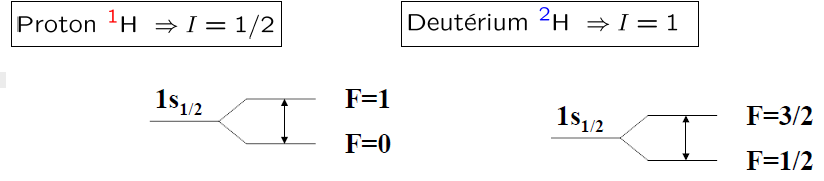
\includegraphics[scale=0.45]{ch1/image12}
\captionof{figure}{Notons pour le $^1$H le bon accord théorie expérience : $v_{th} \approx 1420$ MHz, 
$\nu_{exp} = 1420405751.800$ Hz. Il s'agit de la raie à $\lambda=21$ cm.}
\end{center}

\iffalse



Ca vient du fait que le moment magnétique I aura un moment nucléaire. Il est clolinéaire à mu. . Le rapport entre mu_N et mu_B c'est a peu pres 1836. 

Ici on fait bien un changement d'ECOC en écrivant F=...



\fi